% Official VLDB template: acmart.cls v2.19 (2026/06/27) + pvldb.sty
% (VLDB/PVLDB Vol. 20 formatting overrides). Downloaded from vldb.org.
\documentclass[sigconf, nonacm]{acmart}

%%% do not modify the following VLDB block %%
%%% VLDB block start %%%
\usepackage{pvldb}% VLDB/PVLDB formatting overrides -- do not remove.
%%% VLDB block end %%%

% paper-specific values (placeholders for submission; assigned at production)
\renewcommand\vldbdoi{XX.XX/XXX.XX}
\renewcommand\vldbpages{XXX-XXX}
% supplemental material / artifacts repository (VLDB 2027 Transparency)
\renewcommand\vldbavailabilityurl{https://github.com/1951123/pg-extstats-selection}

% packages useful for this paper
\usepackage{lmodern}
\usepackage{booktabs}
\usepackage{graphicx}
\usepackage{amsmath}
\usepackage{tikz}
\usetikzlibrary{positioning,fit,arrows.meta}

% capacity menu as an in-line-breakable math token (avoids overfull column boxes)
\newcommand{\capmenu}{\{10,\allowbreak 25,\allowbreak 50,\allowbreak 100,\allowbreak 1000,\allowbreak 10000\}}

% let LaTeX stretch lines slightly to absorb long \texttt/numbers near overfull
\emergencystretch=1.5em

\begin{document}

\title{One-Stat Sufficiency Guided Budgeted Selection of PostgreSQL Extended Statistics}

\author{Huiju Wang\textsuperscript{\textdagger}}
\affiliation{%
  \institution{Zhongnan University of Economics and Law}
  \city{Wuhan}
  \country{China}
}
\email{wanghj@zuel.edu.cn}

\author{Jiacheng Lou\textsuperscript{\textdagger}}
\affiliation{%
  \institution{Zhongnan University of Economics and Law}
  \city{Wuhan}
  \country{China}
}
\email{2350353412wqts@gmail.com}

\author{Xiao Yue\textsuperscript{*}}
\affiliation{%
  \institution{Zhongnan University of Economics and Law}
  \city{Wuhan}
  \country{China}
}
\email{yuexiao@zuel.edu.cn}

\author{Yuanfei Sun}
\affiliation{%
  \institution{Zhongnan University of Economics and Law}
  \city{Wuhan}
  \country{China}
}
\email{yfsun@stu.zuel.edu.cn}

\begin{abstract}
Cardinality estimation errors are the main cause of suboptimal execution
plans and performance degradation in PostgreSQL. Multivariate extended
statistics mitigate bias stemming from the column-independence assumption but
demand heavy manual tuning. Existing statistics advisors only select column
combinations (the what dimension), ignoring differentiated sampling-capacity
allocation (the how-much dimension), and cannot balance estimation accuracy
and resource usage under limited storage budgets. Overlapping statistics
further introduce severe planner interference and extra ANALYZE maintenance
costs.
Through extensive workload-driven evaluation, we identify a fundamental
per-query property termed one-stat sufficiency: most single-table queries gain
nearly all possible cardinality improvements from at most one well-chosen
multivariate statistic. For most evaluated queries, additional statistics bring
negligible marginal benefits yet worsen planner interference and maintenance
overhead.
Motivated by this observation, we propose Catalog-Mask, an isolation protocol
that eliminates cross-statistic interference to measure each candidate's
independent storage cost and error-reduction gain. We model statistic tuning as
a budget-constrained integer-programming problem to jointly optimize
column-combination selection and per-statistic sampling-capacity assignment.
Our experiments demonstrate that our method significantly reduces q-error
(the ratio of the planner's estimated to the actual cardinality)
under tight storage budgets while avoiding redundant statistics and planner
interference. We further characterize applicability boundaries and analyze the
mismatch between storage-based budgeting and real-world ANALYZE overhead,
offering empirical support and a practical tuning paradigm for PostgreSQL
extended statistics.
\end{abstract}

\maketitle

{\renewcommand\thefootnote{*}\footnotetext{Corresponding author.}}
{\renewcommand\thefootnote{\textdagger}\footnotetext{These authors contributed equally to this work.}}

%%% do not modify the following VLDB block %%
%%% VLDB block start %%%
\vldbtopmatter
%%% VLDB block end %%%

\section{Introduction}
\label{sec:intro}

Cardinality estimation lies at the heart of relational query optimization.
Inaccurate cardinality estimates frequently produce sub-optimal execution plans
and severely degrade query performance. A major source of estimation error
originates from the ubiquitous column-independence assumption, which ignores
real-world attribute correlations within tables. PostgreSQL provides
multivariate extended statistics including multi-column most-common-value (MCV),
n-distinct, and
functional-dependency statistics to mitigate such bias. Unfortunately, these
statistics require manual identification of correlated column-sets and careful
configuration, imposing heavy tuning burdens on database administrators.

Prior physical-design tools and statistic-recommendation systems automate the
selection of promising column combinations from query
workloads~\cite{chaudhuri1998autoadmin,kraft2004cords}. Nevertheless, existing
solutions suffer from two fundamental limitations. First, they only address the
``what'' dimension: deciding which column-sets should form statistics. Sampling
capacity, which controls estimation quality and storage footprint for each
individual statistic, is treated as a global fixed parameter and never
optimized per candidate. This ``what-only'' strategy cannot realize fine-grained
resource trade-offs under constrained storage budgets. Second, co-deployed
overlapping multivariate statistics introduce negative planner interference,
which distorts cardinality estimates and degrades overall effectiveness.
Without an isolation measurement mechanism, existing work can only observe
aggregated end-to-end quality and cannot quantify the independent benefit of
each candidate statistic. Consequently, interference and redundancy remain
hidden from optimization formulations.

Motivated by this gap, we conduct extensive workload-driven evaluations and
identify an empirical property we term \emph{one-stat sufficiency}. For most
single-table queries, nearly all achievable cardinality-estimation improvement
can be obtained by deploying at most one well-chosen multivariate statistic.
Additional statistics yield negligible marginal gains while amplifying planner
interference and ANALYZE maintenance overhead. This finding reshapes our
understanding of extended-statistics tuning: effective tuning favors
\emph{compact, precise} statistic deployment rather than blindly accumulating
as many statistics as possible.

Measuring independent benefit for each candidate statistic becomes essential
given the above observation, yet simultaneous deployment causes coupled
interference. To tackle this measurement bottleneck, we propose
\emph{Catalog-Mask}, an isolation protocol that eliminates cross-statistic
interference and reliably quantifies the independent storage cost and
error-reduction gain for each candidate column-set. Using the cost-benefit
measurements collected via Catalog-Mask, we formulate statistic tuning as a
budget-constrained integer-programming problem. Our model jointly optimizes two
dimensions: column-combination selection (what) and per-statistic
sampling-capacity assignment (how-much), producing deployments that maximize
overall estimation quality under given storage budgets.

We conduct comprehensive experiments across multiple real and synthetic
workloads. The results demonstrate that our approach substantially reduces
q-error (the ratio of estimated to actual cardinality) and suppresses
redundant, interfering statistics under tight storage
budgets. We explicitly acknowledge an important modeling assumption: our
optimizer uses storage consumption as the budget metric, which exhibits
inherent mismatch against real-world ANALYZE maintenance overhead. We further
characterize applicability boundaries for our technique to avoid over-claiming
its practical scope.

This paper makes the following contributions:
\begin{enumerate}
\item We discover and quantitatively validate the one-stat-sufficiency property
over real-world workloads. Our end-to-end evaluation further highlights the
negative planner-interference effect introduced by co-deployed overlapping
multivariate statistics.
\item We design Catalog-Mask, an isolation protocol that enables reliable
measurement of independent cost-benefit for each candidate statistic, resolving
the coupled-measurement bottleneck.
\item We present a joint what-and-how-much integer-programming formulation,
which simultaneously selects column-sets and assigns differentiated sampling
capacity for PostgreSQL multivariate statistics.
\item We perform extensive end-to-end evaluation, analyze the mismatch between
storage-based budgeting and real ANALYZE maintenance cost, and provide
practical tuning insights for PostgreSQL extended statistics.
\end{enumerate}

\emph{Organization.} The rest of this paper is organized as follows.
\S\ref{sec:back} positions our work against prior physical-design and
statistics-advisor methods. \S\ref{sec:formulation} defines the
budgeted multivariate-statistics selection problem, shows why the general
multi-statistic case is intractable to measure, and derives the
one-stat-sufficiency surrogate that makes the objective exactly linear.
\S\ref{sec:milp} presents our sparse MILP with capacity levels, its
constraints, and solver scalability. \S\ref{sec:measure} introduces the
Catalog-Mask measurement protocol that makes per-candidate, per-capacity
measurement feasible, and validates its correctness. \S\ref{sec:findings}
reports our empirical findings on capacity, one-stat sufficiency, and joint
optimization. \S\ref{sec:e2e} validates the full pipeline on a real database,
exposing and fixing planner interference. \S\ref{sec:disc} discusses
implications, the storage/ANALYZE mismatch, deployment fidelity, and open
questions. \S\ref{sec:concl} concludes.

\section{Background and Related Work}
\label{sec:back}

\subsection{Background}

Cardinality estimation is central to relational query optimization. Estimation
errors often lead to sub-optimal execution plans, largely due to the pervasive
column-independence assumption, which disregards real-world attribute
correlations within tables. To alleviate this bias, PostgreSQL offers
multivariate extended statistics of three types: multi-column MCV,
\texttt{n}-distinct, and functional-\emph{dependency} statistics. This work
focuses solely on MCV-style multivariate statistics intended for single-table
predicates. Such extended statistics apply only to single-relation filter
conditions and cannot directly improve cardinality estimates for join
predicates.

Each multivariate statistic accepts an independent sample-size setting that
governs both its estimation fidelity and storage footprint. PostgreSQL exhibits
an inherent trade-off between per-statistic estimation quality and ANALYZE
maintenance overhead: a larger sample-size setting produces more accurate
estimates. However, ANALYZE runtime is determined by the \emph{maximum}
sample-size setting on the underlying table, instead of summing costs across
individual statistics. Consequently, storage consumption is an additive
resource, while ANALYZE maintenance cost is non-additive.
\emph{This key distinction motivates our choice of storage consumption as the
primary budget metric for statistic tuning}.

Although these configuration knobs are available, PostgreSQL multivariate
extended statistics still demand manual discovery of correlated column-sets and
manual adjustment of sample-size settings, placing significant operational
burden on database administrators.

\subsection{Related Work}

Physical database design has extensively investigated workload-driven selection
of auxiliary structures such as indexes and materialized views under explicit
space budgets~\cite{agrawal2000automated}. Classic AutoAdmin solutions cast
physical design as a budget-constrained combinatorial optimization and adopt
what-if interfaces to estimate candidate benefits without actual
deployment~\cite{chaudhuri1997efficient,chaudhuri1998autoadmin}. Subsequent work
further generalized physical-design search frameworks to support rich
constraints, including update-driven maintenance overhead for physical
structures~\cite{bruno2005automatic,bruno2010constrained}. A widely-adopted
implicit assumption within these physical-design solvers is that the benefit
contributed by each physical object is approximately independent when multiple
objects co-exist. Nevertheless, multivariate extended statistics in PostgreSQL
exhibit negative interference: overlapping co-deployed statistics may mislead
the query planner and degrade cardinality estimation quality, a side-effect
that does not arise for index selection.

A large body of work studies multidimensional summaries and
cardinality-estimation mechanisms, including multi-dimensional histograms,
compact sketches, and learned estimators~\cite{bruno2001stholes,negi2023robust,kipf2018learned}.
These efforts mostly focus on designing novel summary structures or replacing
the optimizer's internal estimation logic. By contrast, our work reuses
PostgreSQL's native multivariate statistics (MCV, ndistinct,
functional-dependency statistics), and addresses the \emph{deployment} problem:
selecting appropriate column-sets and assigning per-object sampling capacity,
rather than inventing new statistic representations.

Multiple industrial and research prototypes support automatic
multivariate-statistic recommendation. The CORDS prototype extracts column
correlation and generates candidate statistics guided by workload
predicates~\cite{kraft2004cords,ilyas2004cords}. Haas et al.\ propose an
alternative feedback-driven approach to detect attribute dependencies from
query execution traces~\cite{haas2007detecting}. Early work on automated
statistics management focuses on pruning redundant candidate statistics for
workloads, but does not tune per-object sampling resolution~\cite{chaudhuri2001automating}.
Production PostgreSQL advisors --- EDB's Statistics Advisor~\cite{edb_query_advisor}
and pg\_qualstats~\cite{pg_qualstats} --- as well as SQL Server's built-in
tooling recommend promising column combinations derived from query predicates.
All these existing solutions solve only the ``what'' dimension of statistic
selection: they treat per-statistic sampling capacity as a global fixed
parameter and never optimize it for individual candidates. Moreover, prior
approaches evaluate end-to-end estimation quality after deploying an entire set
of statistics, lacking isolation mechanisms to quantify the independent benefit
of each candidate statistic. Consequently, planner interference is not modeled,
and redundancy caused by overlapping statistics stays concealed from
optimization formulations.

Table \ref{tab:taxonomy} situates our contribution against this lineage.

\begin{table*}[t]
\caption{Positioning against automatic statistics configuration.
\checkmark\;\,= yes, \;$\sim$\;= partial, -- = no/depends.}
\label{tab:taxonomy}
\small
\begin{tabular}{lccccccc}
\toprule
 & \shortstack[c]{candidate\\discovery} & \shortstack[c]{multivariate\\statistics} & \shortstack[c]{workload\\driven} & \shortstack[c]{budget\\unit} & \shortstack[c]{capacity\\tuning} & \shortstack[c]{PostgreSQL} & \shortstack[c]{E2E\\planner validation}\\
\midrule
Chaudhuri \& Narasayya & \checkmark & -- & \checkmark & storage & -- & -- & --\\
CORDS \cite{ilyas2004cords} & \checkmark & $\sim$(pair) & -- & catalog & -- & -- & --\\
Haas et al.\ \cite{haas2007detecting} & \checkmark & $\sim$(pair) & \checkmark & catalog & -- & -- & --\\
EDB Statistics Advisor \cite{edb_query_advisor} & \checkmark & $\sim$($\le$2 col) & \checkmark & weighting & $\sim$ & \checkmark & --\\
pg\_qualstats \cite{pg_qualstats} & \checkmark & -- & \checkmark & -- & -- & \checkmark & --\\
\textbf{This work} & \checkmark & MCV & \checkmark & \textbf{storage} & \checkmark & \checkmark & \checkmark\\
\bottomrule
\end{tabular}
\end{table*}

\section{Problem Formulation}
\label{sec:formulation}

This section defines the cardinality-estimation optimization problem for
budgeted multivariate-statistics selection. We first introduce notation and the
objective function (\S\ref{sec:notn}); we then show the intrinsic difficulty of
the general multi-statistic selection problem (\S\ref{sec:multi}); next we
introduce the empirical one-stat-sufficiency property and derive its
consequence, an exactly-linear surrogate model (\S\ref{sec:sparse}); and we
close by highlighting the measurement bottleneck (\S\ref{sec:measure}) that
motivates our measurement infrastructure.

\subsection{Notation and Objective}
\label{sec:notn}

\begin{center}\small
\begin{tabular}{@{}l@{\hspace{1.2em}}p{0.62\columnwidth}@{}}
\toprule
Symbol & Meaning\\
\midrule
$Q=\{q_1,\dots,q_n\}$, $n$ & workload of $n$ queries; $q_i$ is the $i$-th query\\
$e_i^0$ & baseline q-error of $q_i$ with no extended statistics\\
$e_{is}$ & q-error of $q_i$ when it uses only physical statistic $s$\\
$s=(t,\mathrm{cols},L)$ & a physical statistic (table $t$, a column set, capacity level $L$)\\
$c_s$ & persistent storage cost of statistic $s$ (bytes)\\
$C$ & storage budget\\
$y_s$ & $1$ if statistic $s$ is created, otherwise $0$\\
$x_{is}$ & $1$ if query $q_i$ is assigned statistic $s$, otherwise $0$\\
$T_i$ & the set of created statistics used by $q_i$\\
$\Delta_{is}=e_i^0-e_{is}$ & per-query improvement from statistic $s$ on $q_i$\\
\bottomrule
\end{tabular}
\end{center}

We are given a workload of queries $Q=\{q_1,\dots,q_n\}$. The accuracy of the
planner's estimate for $q_i$ is the \textbf{q-error}
\[
  \operatorname{qerr}(\text{est},\text{act})=\frac{\max(\text{est},\text{act})}
  {\min(\text{est},\text{act})}\ge 1.
\]
Let $e_i^0$ be the baseline q-error of $q_i$ with no extended statistics. A
\emph{physical statistic} is $s=(\text{table},\text{columns},\text{level})$,
with storage cost $c_s$ (bytes) and a per-query effective q-error $e_{is}$
when $q_i$ uses only $s$.

\emph{Why a storage budget.} We deliberately optimize \emph{persistent
storage} $c_s$ rather than \texttt{ANALYZE}/maintenance time. PostgreSQL couples
sampling effort to the \emph{maximum} statistics target on a relation, so
maintenance cost is not a per-statistic additive quantity that any selection
model can budget over; storage, by contrast, is a clean additive resource that
every selected statistic consumes and that competes for a shared budget
(\S\ref{sec:mechanisms}). We therefore frame the problem as \emph{storage-budgeted
selection} and treat maintenance-aware optimization as a separate extension
(\S\ref{sec:disc-objective}). The selection objective is
\[
  \min_{\{y_s\},\{x_{is}\}}\; \frac{1}{n}\sum_i \operatorname{qerr}_i\big(T_i\big)
  \quad\text{s.t.}\quad \sum_s c_s\,y_s \le C,
\]
where $y_s\in\{0,1\}$ says statistic $s$ is created and $T_i$ is the set of
created statistics used by $q_i$. Because a statistic can serve many queries,
we use the assignment $x_{is}\le y_s$ so each \emph{physical} object is built
once and its storage paid once in the budget --- the shared-resource semantics
that make global selection different from per-query greedy.

\subsection{The General Multi-select Problem Is Intractable to Measure}
\label{sec:multi}

Read naively, the objective over $T_i$ is a \emph{combinatorial} problem: each
query could use any subset of its candidate statistics, and the joint q-error
$e_i(T_i)$ of a \emph{set} $T_i$ depends on how those statistics interact in the
planner. Optimizing over $\{y_s\}$ then requires knowing $e_i(T)$ for arbitrary
subsets --- which in general cannot be composed from the per-statistic values
$e_{is}$. Even \emph{measuring} all subsets is infeasible, let alone optimizing
over them.

A standard workaround is the multiplicative approximation in log space
\cite{ioannidis2003history},
\[
  \log e_i(T_i)\;\approx\;\log e_i^0 + \sum_{s\in T_i}\log\!\Big(\tfrac{e_{is}}{e_i^0}\Big),
\]
which treats each statistic's contribution as independent. This is exact only
when the chosen statistics act independently, and can break when overlapping
statistics coexist (we return to this in \S\ref{sec:e2e}).

\subsection{One-Stat Sufficiency: An Exactly-Linear Special Case}
\label{sec:sparse}

Our measurements (\S\ref{sec:rq1}) reveal that per query a
\emph{single dominant statistic} already captures nearly all improvement
attainable from the evaluated 2-/3-column MCV candidates, which motivates a
\emph{restricted} model: a budgeted statistic-selection problem in which each
query selects at most one statistic, $\sum_s x_{is}\le 1$. This \emph{one-stat
sufficiency} is \emph{empirically justified}, not a modeling assumption that
holds by definition: it is exact conditional on the one-statistic-per-query
regime, and \S\ref{sec:rq1} characterizes when that regime holds and when it
fails. Within it, the restriction removes the interaction that makes the general
problem hard: with at most one statistic per query, $e_i(T_i)$ is either $e_i^0$
(no statistic) or $e_{is}$ (the single selected statistic), so no joint term
arises.

\begin{proposition}[Exact linearity of the singleton-effect surrogate]
\label{prop:linear}
Consider the \emph{surrogate} model in which a query's error is $e_i^0$ if no
statistic is assigned and $e_{is}$ if it is assigned the single statistic $s$
(i.e.\ the per-query error \emph{as the model computes it}, not necessarily what
the real planner produces). If each query is assigned at most one statistic
($\sum_s x_{is} \le 1$), then the surrogate objective is exactly
\[
  e_i\big(T_i\big)\;=\;e_i^0\;-\;\sum_s \big(e_i^0-e_{is}\big)\,x_{is},
\]
with no interaction term, so the surrogate workload objective is linear in the
selection variables.
\end{proposition}
\begin{proof}[Proof sketch]
For a fixed query $i$, $T_i$ is either empty (surrogate error $e_i^0$) or a
singleton $\{s\}$ (surrogate error $e_{is}$); since at most one $x_{is}$
equals $1$, no two statistics co-occur, so no joint term arises and the
objective is linear. This is a statement about the \emph{model}; whether the
real planner reproduces $e_{is}$ for the chosen $s$ is a separate, empirical
question answered by the end-to-end (E2E) validation (\S\ref{sec:e2e}).
\end{proof}

The log-space approximation is therefore unnecessary for the sparse surrogate;
we solve the linear form exactly. This is the sense in which the integer program
promised in the introduction (\S\ref{sec:intro}) specializes here: one-stat
sufficiency removes the interaction term, so the general program degenerates to
an \emph{exactly linear} mixed-integer linear program (MILP) under the
singleton-effect restriction, and
\S\ref{sec:p1} then determines when that surrogate stays faithful to
PostgreSQL's actual selection after deployment. We call this the \emph{capacity-aware} selection problem: because
each capacity level is a distinct physical statistic, choosing \emph{which}
level of a combination to build is expressed by selecting the corresponding
$y_{(table,cols,level)}$, subject to a global budget.

\paragraph{Measurement bottleneck.}
The sparse integer program developed in \S\ref{sec:milp} requires
per-candidate, per-capacity inputs for every candidate statistic $s$: its
storage cost $c_s$ and its isolated q-error $e_{is}$. These values cannot be
obtained trivially from vanilla PostgreSQL; a naive create-analyze-drop cycle is
computationally prohibitive on wide tables with large candidate pools. We
resolve this bottleneck in \S\ref{sec:measure} with the Catalog-Mask isolation
protocol.

\section{Optimization: Sparse MILP with Capacity Levels}
\label{sec:milp}

This section presents our sparse mixed-integer linear programming (MILP)
formulation for capacity-aware extended-statistics selection. Building on the
one-stat-sufficiency surrogate (\S\ref{sec:sparse}), we maximize total error
reduction under a global storage budget. We describe the decision variables and
objective, the constraints (including an optional deployment-aware variant),
and pruning and solver scalability (\S\ref{sec:scale}); the MILP consumes the
per-candidate cost-benefit measurements $(c_s,e_{is})$ produced by the
measurement infrastructure of \S\ref{sec:measure}.

\subsection{Variables and Objective}

The MILP decides \emph{which physical statistics to build}; the variables are
$y_s$ (create physical statistic $s$) and $x_{is}$ (query $i$ uses $s$ in the
surrogate, of \S\ref{sec:sparse}). By Prop.~\ref{prop:linear}, minimizing mean
q-error is equivalent to maximizing total improvement,
\[
  \max \sum_{i,s}\underbrace{\big(e_i^0-e_{is}\big)}_{\Delta_{is}\ge 0}x_{is},
\]
where an option with $\Delta_{is}\le 0$ (no better than baseline) is pruned in
advance.

\subsection{Constraints}

The MILP enforces: (1) the storage budget $\sum_s c_s y_s\le C$; (2) a statistic
must exist to be used, $x_{is}\le y_s$ (shared across queries); (3) sparse
per-query cap $\sum_s x_{is}\le 1$; and (4) capacity-level exclusivity
$\sum_{\ell} y_{(cols,\ell)}\le 1$ (one level per column-combination). A fifth,
optional constraint enforces \emph{global column disjointness}: $y_a+y_b\le 1$
when the column sets of $a,b$ overlap. We support two solver variants. The
\emph{disjoint-set variant} enables this optional constraint, producing
pairwise column-disjoint statistic sets whose per-candidate predictions compose
after deployment (\S\ref{sec:p1}), at a quantified nominal-quality cost; the
\emph{unconstrained variant} omits it, optimizing the surrogate more
aggressively but allowing overlapping statistics whose joint planner effect must
be checked at deployment.

\textbf{Remark.} We defer the names ``Option-A'' and ``Option-B'' for these two
deployment modes to \S\ref{sec:disc-fix}, after presenting end-to-end
deployment evidence; we avoid introducing these aliases before the experimental
results motivate them.

\subsection{Pruning and Solve Scalability}
\label{sec:scale}

Two factors keep the MILP small. First,
\texttt{skip\_}\allowbreak\texttt{worse\_}\allowbreak\texttt{than\_baseline}
drops any option whose per-query q-error is not better than the no-stat
baseline; because baseline estimates are usually already good, most options are
pruned, leaving only genuine ``repairers''. Second, global deduplication means
$n_{\text{stats}}$ is the deduplicated universe of
$(\text{table},\text{cols},\text{level})$ rather than the per-query sum. On the
full 468-query CENSUS workload the resulting problem is large but trivially
solvable: the worst-case (no pruning) instance over the full six-level menu
$\capmenu$ has 115{,}470 physical
statistics, 185{,}136 options and 300{,}606 binary variables and is solved
optimally by HiGHS in $\approx$4.0s; with pruning it shrinks to 69{,}431
statistics / 89{,}727 options / 159{,}158 variables ($\approx$2.8s). Thus the
optimization is not the bottleneck at full-workload scale --- the phase-1
\emph{measurement} is (\S\ref{sec:measure}).

\section{Measurement Infrastructure}
\label{sec:measure}

As established in \S\ref{sec:milp}, our sparse MILP requires per-candidate,
per-capacity measurements: the on-disk storage cost $c_s$ and the isolated
q-error $e_{is}$ for every physical statistic
$s=(\texttt{table},\texttt{columns},\texttt{level})$. We take $c_s$ as the
serialized MCV payload in the \texttt{stxmcv} column of
\texttt{pg\_statistic\_ext\_data} (read via
\texttt{pg\_column\_size}\allowbreak), so a coarser capacity is simply a smaller
list, and out-of-line (TOAST) storage is counted by the same call. A naive
create-analyze-drop cycle is computationally intractable on wide tables with
large candidate pools, so we need an efficient isolation protocol. This section
introduces \emph{Catalog-Mask (Protocol-M)}: we first recap relevant PostgreSQL
internals (\S\ref{sec:mechanisms}), demonstrate the infeasibility of naive
measurement (\S\ref{sec:measure-naive}), describe the protocol
(\S\ref{sec:measure-mask}), validate its correctness (\S\ref{sec:measure-correct}),
and analyze measurement cost and granularity (\S\ref{sec:measure-runtime}).

\subsection{Internal Semantics of PostgreSQL Extended Statistics}
\label{sec:mechanisms}

Several mechanism facts (verified from the PostgreSQL 16 source) ground the
model. \textbf{Scope.} Extended statistics are consulted only for
\emph{restriction} (WHERE) clauses on a \emph{single relation}: the selectivity
entry point is gated by a single-relation check, and \texttt{eqjoinsel} never
consults \texttt{pg\_statistic\_ext}. Consequently extended statistics do not
directly estimate cross-relation join selectivity --- they act on single-table
restriction clauses, so their direct effect is confined to single-relation
selection predicates (they can influence a join plan only indirectly, through
base-cardinality estimates). This is why our evaluation separates single-table
workloads (where they act directly) from join workloads (a negative control).

\textbf{Capacity is per-object and tunable.} Each statistic can be assigned its
own \texttt{statistics\_}\allowbreak\texttt{target} via \texttt{ALTER STATISTICS}\allowbreak\texttt{ \dots\ SET STATISTICS}
(stored in \texttt{stxstattarget}). The ANALYZE sampling effort is coupled to the
\emph{largest relevant statistics target} on the relation (including the
extended statistics' own targets) \cite{pgstats}; consequently, raising an
extended-statistics target can increase maintenance cost beyond the persistent
storage cost our objective models (\S\ref{sec:measure-naive}). Because of this
coupling we deliberately optimize a \emph{storage} budget --- the persistent
bytes of the selected statistics and the estimation quality they deliver --- and
treat ANALYZE maintenance cost separately (it is a property of the maximum, not
the sum, of targets).

\textbf{Capacity-quality trade-off.} \texttt{statistics\_target} is the knob
that sets an extended statistic's precision: for an MCV statistic it caps how
many most-common value-tuples the list stores, and it scales ANALYZE's
sampling effort (\cite{pgstats}). It is a \emph{cap}, not a requirement: a
column-combination with fewer frequent tuples than the cap is fully captured at
any larger target, so raising the target helps only while the list is
\emph{target-capped} (still filling) rather than \emph{data-capped} (bounded by
the data's own cardinality). Capacity is therefore a two-sided allocation axis
--- \emph{raising} it resolves target-capped combinations, \emph{lowering} it
saves storage on data-capped ones --- which is why \emph{how much} must be
decided jointly with \emph{which} statistics under a shared budget
(\S\ref{sec:rq4}). We model capacity as a menu of levels spanning both
directions of this axis, anchored on the default 100 and extending below and
above it (the exact menu is in \S\ref{sec:findings}).

\subsection{Infeasibility of Naive Measurement on Wide Tables}
\label{sec:measure-naive}

The obvious protocol (\emph{Protocol-A}) isolates a candidate by
\[
  \begin{aligned}
    \text{CREATE} &\to \text{ANALYZE}\\
    &\to \text{EXPLAIN} \to \text{DROP} \to \text{ANALYZE},
  \end{aligned}
\]
a clean, drop-analyzable cycle that costs two ANALYZEs per candidate. On a wide
table this is prohibitive. On the CENSUS \texttt{climate} table (69 columns,
$\sim$2.5M rows) a single ANALYZE at \texttt{statistics\_target}\allowbreak$=10000$ takes
$\approx$22s with no statistics (warm cache; a fixed base cost), growing
roughly linearly with the number of statistics already on the table
(\S\ref{sec:measure-runtime}). Consequently the naive protocol
costs $\approx$44s per candidate --- two ANALYZEs $\times$ $\approx$22s. Even
after deduplication the full workload leaves 19{,}245 distinct candidates, so
Protocol-A would need $\approx$9.8 days of ANALYZE time at this capacity alone
--- not a tractable phase-1.

Crucially, this infeasibility is \emph{not} an accident of an arbitrarily
large menu: the $\approx$22s per-ANALYZE base cost is the necessary
consequence of fixing the single-column statistics at a generous target so
that the baseline is fixed and reproducible --- a comparability requirement,
not a claim of exact determinism given ANALYZE's sampling
(\S\ref{sec:measure-determinism}). One cannot buy it away by shrinking the
target without sacrificing that reproducibility. Protocol-M is therefore the
mechanism that makes a principled (expensive-but-stable) measurement
tractable, rather than a way to paper over an unnecessarily high cost.

\subsection{The Catalog-Mask Protocol (Protocol-M)}
\label{sec:measure-mask}

Our \textbf{catalog-mask protocol} builds all of a table's candidate statistics
\emph{once}, in a single ANALYZE (sampled at the maximum target), and measures
each candidate in isolation by \emph{masking} the others (Fig.~\ref{fig:mask}).
Masking NULLs the
other candidates' payload in \texttt{pg\_statistic\_ext\_data}; the planner's
\texttt{statext\_is\_kind\_built()} test then omits a NULL-payload statistic from
\texttt{rel->statlist}, so the planner behaves as if that statistic did not
exist --- an implementation-exact isolation for PostgreSQL 16 that costs no
ANALYZE. Payloads are restored from a
temporary backup table via \texttt{UPDATE ... FROM} (the \texttt{pg\_mcv\_list}
type has no bytea cast, so the round-trip must happen inside the server).
Multiple capacity levels are measured with one object per (candidate, level)
via \texttt{ALTER STATISTICS}\allowbreak\texttt{ \dots\ SET STATISTICS}, again built by a single
ANALYZE at the maximum target. Protocol-M therefore replaces two ANALYZEs per
candidate with \emph{one} mask--EXPLAIN--restore cycle per candidate, whose cost
is dominated by the catalog UPDATE and grows with the number of payloads
mounted on the table (a tunable granularity; \S\ref{sec:measure-runtime}) ---
not by a fixed EXPLAIN. The saving is about amortizing the fixed ANALYZE
base cost (\S\ref{sec:measure-runtime}): a table's sample and per-column
statistics are recomputed on every ANALYZE, so Protocol-A pays that base twice
per candidate, whereas Protocol-M pays it once per batch of candidates.

\begin{figure*}[t]
\centering
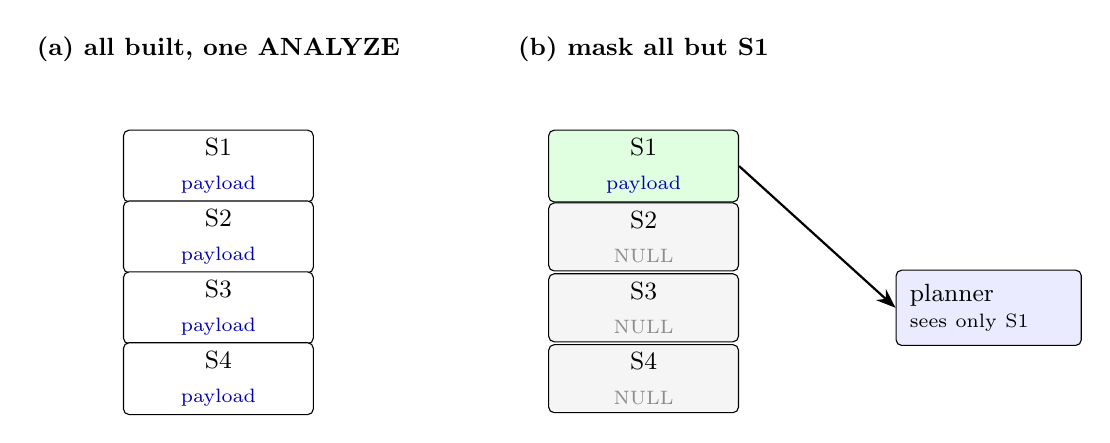
\begin{tikzpicture}[
  stat/.style={draw, rounded corners=2pt, inner sep=3pt, font=\small,
               text width=22mm, align=center},
  pay/.style={text=blue!70!black},
  null/.style={text=black!45},
  arr/.style={-{Stealth[length=2.5mm]}, thick}
]
% ---- left: all built ----
\node[font=\small, anchor=south] at (0,1.2) {\textbf{(a) all built,\ one ANALYZE}};
\foreach \i/\nm in {0/S1,1/S2,2/S3,3/S4}{
  \node[stat, fill=white] (l\i) at (0,-0.9*\i) {\nm\\[0.5mm]{\scriptsize\color{blue!70!black}payload}};
}
% ---- right: masked (S1 measured) ----
\node[font=\small, anchor=south] at (5.4,1.2) {\textbf{(b) mask all but S1}};
\node[stat, fill=green!12] (r0) at (5.4,0.0)  {S1\\[0.5mm]{\scriptsize\color{blue!70!black}payload}};
\foreach \i/\nm in {1/S2,2/S3,3/S4}{
  \node[stat, fill=black!4] (r\i) at (5.4,-0.9*\i) {\nm\\[0.5mm]{\scriptsize\color{black!45}NULL}};
}
% ---- planner box (right of the masked list) ----
\node[draw, rounded corners=2pt, fill=blue!8, inner sep=5pt, font=\small,
      anchor=west, text width=20mm] (pln) at (8.6,-1.8)
      {planner\\[-0.5mm]{\scriptsize sees only S1}};
\draw[arr] (r0.east) -- (pln.west);
\end{tikzpicture}
\caption{The catalog-mask protocol (Protocol-M): all candidates are built in one
ANALYZE, and each is measured by NULLing the others' payloads so that the
planner sees only it, via a mask--EXPLAIN--restore cycle
(\S\ref{sec:measure-runtime}) rather than an ANALYZE.}
\label{fig:mask}
\end{figure*}

\subsection{Correctness of Masked Measurement}
\label{sec:measure-correct}

Masking must reproduce what a \emph{single} deployed statistic would deliver.
We validate this directly by measuring each candidate's q-error twice: (i)
\emph{singleton}, building only that statistic, and (ii) \emph{masked}, building
the candidate plus three overlapping siblings in one ANALYZE and NULLing the
siblings' payloads. The two agree to the last digit every time --- e.g.\
\texttt{FavCnt+ViewCnt} and \texttt{AnsCnt+ViewCnt} at L10000 both read
1.0012 and 1.0129 singleton vs.\ masked; st.144 masked 1.04 vs.\ singleton
1.042 (\S\ref{sec:e2e}). Together with the fact that a NULL payload is ignored
by the planner, this confirms Protocol-M is an \emph{exact} isolation of each
candidate's effect -- not an approximation.

\textbf{Pragmatics and scope.} Protocol-M writes the system catalog directly,
so the manipulation runs in a dedicated, disposable cluster (or with autovacuum
and concurrent writes suspended); standard cache invalidation keeps every
\texttt{EXPLAIN} fresh, and NULLing a payload does not re-run ANALYZE, so
masking cost is independent of table size (full safeguards in the artifact).
Two limits are honest implementation constraints rather than model choices:
Protocol-M relies on the system-catalog layout and the planner's
object-identifier (OID) order
selection (\S\ref{sec:switch}), so it is specific to PostgreSQL 16 and to
\emph{MCV} statistics (\S\ref{sec:disc-objective}). Its advantage grows with
dataset scale --- the classical per-candidate ANALYZE pays the table's fixed
base cost twice per candidate, Protocol-M pays it once per batch
(\S\ref{sec:measure-runtime}) --- so at multi-hundred-GB scale Catalog-Mask
becomes the \emph{only} tractable path (\S\ref{sec:measure-naive}).

\subsection{Measurement Cost and Granularity}
\label{sec:measure-runtime}

\emph{Deterministic single-column baseline.}\label{sec:measure-determinism}
Because \texttt{ANALYZE} is sampling-based, we fix the per-column
\texttt{statistics\_target} at 10000 rather than PostgreSQL's default of 100:
it removes run-to-run drift (reproducible, coefficient of variation
(CV)~$0$), avoids \emph{empty}
high-capacity payloads that would degrade the baseline, and attributes any
extended-statistic gain purely to correlation rather than to patching a coarse
per-column estimate. All per-candidate q-errors $e_{is}$ are measured against
this \emph{same} baseline, so capacity is the only axis that changes between
levels. This makes a wide-table single-column ANALYZE \emph{expensive} (a CENSUS
ANALYZE at target\,10000 costs $\approx$22\,s), precisely what forces the
catalog-mask protocol (\S\ref{sec:measure-naive}, \S\ref{sec:measure-mask}) ---
the large fixed target and Protocol-M are two halves of one design decision.

\emph{Protocol-M is a large-sample oracle, not a deployment emulator.}
Fixing the single-column baseline at a generous target means every capacity
level $L$ is evaluated on the same \emph{large} sample ($\sim$3M rows), even
though a real ``\texttt{SET STATISTICS} $L$'' deployment builds that candidate
on the smaller sample its own target implies. Protocol-M thus measures a
\emph{conditional large-sample oracle} view $e_{is}(L)$, which isolates capacity
as the only axis (\S\ref{sec:measure-determinism}) but is not a claim that real
deployment reproduces it exactly; we assess deployment fidelity in
\S\ref{sec:disc-deployment}. Note that the fixed target\,10000 baseline is a
\emph{measurement-design baseline, not a deployment recommendation} --- a
real deployment need not raise any single-column target.

\emph{Batch granularity.}
Masking rewrites the catalog, so a masked measurement is \emph{not} constant:
its cost grows with the number of payloads mounted during that measurement, a
property of the measurement \emph{granularity} rather than of Protocol-M per se.
Grouping candidates into batches therefore amortizes the fixed per-batch ANALYZE
base but lengthens each mask, so the total is convex in batch size with a
workload-dependent optimum (Tab.~\ref{tab:measurement}); a closed-form optimum
and the full timing model are deferred to the artifact. The optimum grows with
the ANALYZE base and shrinks as masking or sharing rises, so a workload-wide
build is optimal only under very high sharing; on CENSUS we sub-batch instead,
splitting candidate-dense queries into $\approx$55-candidate sub-batches. On the
most candidate-dense CENSUS query (\texttt{query.335}, $n{=}455$) sub-batching
cuts measurement from $181.4$\,s to $63.4$\,s ($2.9\times$). Against
Protocol-A's per-candidate cost the measured speedup is $\approx$283$\times$ on
CENSUS and $\approx$36$\times$ on \texttt{stats\_CEB\_single} (lower bounds,
since Protocol-A's per-candidate \texttt{ANALYZE} is no more than the table's
base). Thus Catalog-Mask --- not the MILP --- is the enabling component that
makes the candidate $\times$ capacity space measurable.

\begin{table*}[t]
\caption{Measurement cost vs.\ sub-batch size $b$ on one candidate-dense query
per workload.}
\label{tab:measurement}
\small
\begin{tabular}{lcccc@{\hskip 6pt}lcccc}
\toprule
\multicolumn{5}{c}{CENSUS \texttt{query.3}\ ($nL{=}504$)} &
\multicolumn{5}{c}{\texttt{stats\_CEB\_single} \texttt{st.144}\ ($nL{=}210$)}\\
\cmidrule(lr){1-5}\cmidrule(lr){6-10}
sub-batch $b$ & \emph{size} $s$ & total & ANALYZE & mask &
sub-batch $b$ & \emph{size} $s$ & total & ANALYZE & mask\\
(no.) & (cands) & (s) & (s) & (s) &
(no.) & (cands) & (s) & (s) & (s)\\
\midrule
\textbf{1} & \textbf{504} & \textbf{402.0} & 210.3 & 186.0 &
1 & 210 & 47.9 & 4.0 & 37.5\\
3 & 168 & 496.9 & 435.9 & 57.9 &
2 & 105 & 27.7 & 5.9 & 18.3\\
7 & 72 & 938.2 & 910.3 & 25.4 &
\textbf{4} & \textbf{52} & \textbf{22.2} & 10.1 & 8.9\\
14 & 36 & 1646.0 & 1631.4 & 12.3 &
7 & 30 & 23.3 & 15.9 & 5.1\\
28 & 18 & 3398.9 & 3390.4 & 6.3 &
10 & 21 & 27.3 & 22.9 & 3.4\\
\bottomrule
\end{tabular}

{\footnotesize $nL$ = distinct (candidate$\times$level) objects}
\end{table*}

\section{Experimental Evaluation}
\label{sec:evaluation}
\label{sec:findings}

This section evaluates the effectiveness of our what-and-how-much MILP formulation under ideal interference-free conditions obtained from Catalog-Mask measurements. Real-system deployment artifacts such as planner interference caused by overlapping co-installed statistics and our two deployment strategies (Option-A, Option-B) are analyzed separately in Section~\ref{sec:end2end}.

\begin{quote}
All measurements in this section are obtained via the Catalog-Mask large-sample oracle protocol, representing upper-bound estimation quality. Sampling fidelity under real deployment is discussed in \S\ref{sec:disc-deployment}.
\end{quote}

We formulate four research questions to guide our evaluation:
\begin{itemize}
    \item \textbf{RQ1}: To what extent does the one-stat-sufficiency property hold over real-world workloads? Under which conditions does this empirical property break down?
    \item \textbf{RQ2}: Compared against practical naive-tuning and algorithmic baselines, how much Q-error reduction can our joint what-and-how-much optimization achieve under different storage-budget constraints?
    \item \textbf{RQ3}: What performance benefit originates from the how-much dimension? How does our full model compare against a what-only ablation that uses a fixed global sample-size?
    \item \textbf{RQ4}: How sensitive is the output quality and statistic composition of our MILP solution to changes in the input storage budget?
\end{itemize}

\subsection{Experimental Setup}
\label{sec:setup}

\subsubsection{Datasets and Workloads}
We conduct our primary evaluation on two real-world single-table query workloads: \textsc{Census} and \textsc{stats-CEB-single}. Join-related predicates are excluded from evaluation because PostgreSQL multivariate MCV statistics cannot directly improve join cardinality estimates.

\textsc{Census} evaluates the wide \texttt{climate} table (69 columns,
$\sim$2.5M rows) under 468 selection queries drawn from the US Census 1990 task;
\textsc{stats-CEB-single} evaluates the single-table sub-plans of the
StackExchange \textsc{stats-CEB} benchmark (632 queries over 6 small-to-medium
relations, $\le$328K rows). For each query we generate as candidate statistics
the 2-/3-column subsets of its filter predicates --- they directly exercise
single-relation correlation while keeping the candidate space tractable.
Candidates that carry no filter predicate are excluded from aggregation.
Table~\ref{tab:bench} summarizes the workloads and candidate distribution.

\begin{table*}[t]
\caption{Workload characteristics and candidate distribution.}
\label{tab:bench}
\small
\begin{tabular}{lcccl@{\hskip 3pt}c}
\toprule
benchmark & queries & \shortstack[c]{candidates\\per query (total)} & \shortstack[c]{queries\\with any\\candidate} & \shortstack[c]{global\\distinct} & \shortstack[c]{per-query\\min/p25/med/p75/max} \\
\midrule
CENSUS            & 468 & 30856 & 467 & 19245 & 0/20/56/84/455\\
stats\_CEB\_single & 632 & 616   & 180 & 78    & 0/0/0/1/35\\
stats\_CEB (join) & 146 & 616   & 111 & 78    & 0/1/2/5/39\\
job-light (join)  & 70  & 5     & 5   & 1     & 0/0/0/0/1\\
\bottomrule
\end{tabular}
\end{table*}

In addition, we construct synthetic stress-test workloads. These synthetic instances are manually crafted to contain multiple independent attribute-correlation clusters and serve exclusively for probing the failure boundary of one-stat sufficiency.
Synthetic workloads are not representative of typical real-world schema and predicate patterns.
We do \textbf{not} execute the complete tuning pipeline over these synthetic instances for end-to-end quality comparison.

Concretely, the synthetic table \texttt{syn\_clusters} (100K rows) contains
$K$ pairwise \emph{independent} groups of perfectly-correlated columns (each
group $G_j$ over 3 columns), plus an independent filler column; a query then
filters on one attribute from each of $K$ groups simultaneously (``$K$
independent correlated clusters''). As $K$ grows, the number of independent
dominant statistics a single query needs grows with it, letting us probe
exactly where one-stat sufficiency must fail.

\subsubsection{Baselines}
We compare against the following baselines under identical storage-budget constraints.
All competing approaches are strictly enforced to respect the same storage upper bound for fair comparison.
\begin{enumerate}
    \item \textbf{No-stats}: Native PostgreSQL without any multivariate extended statistics; serves as a low-quality reference point.
    \item \textbf{All-default-candidates}: A naive DBA-oriented practical baseline. We construct every candidate multivariate statistic extracted from query predicates with PostgreSQL's default global sample-size of 100. It mimics the ``build-as-many-stats-as-possible'' manual tuning practice.
    \item \textbf{What-only ablation}: Our MILP formulation with the how-much dimension disabled. Only column-set candidates are selected; every selected statistic is assigned a uniform fixed sample-size. This baseline isolates quality gains brought by differentiated per-statistic sample-size allocation.
    \item \textbf{Greedy-baseline}: A knapsack-style marginal-benefit greedy heuristic (variant G2). It consumes exactly the same Catalog-Mask-measured cost-benefit tuples as our MILP solver. Alternative greedy variants (G1, G3) are presented in supplementary material.
\end{enumerate}

\begin{quote}
\noindent\textbf{Note on existing tooling:}
EDB Statistics Advisor is proprietary software tightly coupled to EDB Postgres Advanced Server and cannot run on community PostgreSQL 16.14.
\texttt{pg\_qualstats} acts purely as a predicate-trace collector and implements no automatic statistic recommendation logic.
Neither tool can produce statistic sets subject to our combined constraints of storage budget and per-statistic capacity assignment, so apples-to-apples experimental comparison is technically infeasible.
\end{quote}

The \texttt{What-only ablation} fixes every selected statistic at sample size
\texttt{100} (PostgreSQL's default) --- the fixed uniform sample size used
throughout. The \texttt{Greedy} baseline (G2) iteratively picks the statistic
with the highest marginal improvement-per-storage-byte across still-unserved
queries, always within budget; variants G1 and G3 are detailed in the
supplemental material. All baselines --- like the MILP --- are evaluated on the
Catalog-Mask-measured cost-benefit tuples (\S\ref{sec:measure}), so the only
difference is the selection algorithm, not the measurement.

\subsubsection{Metrics and Implementation Details}
Our primary aggregated evaluation metric is the \textbf{geometric mean of per-query q-error} across evaluated single-table predicates.
Queries without filter predicates are excluded from aggregation.
Since geometric mean can obscure catastrophic estimation outliers, we additionally report \textbf{P90 and maximum q-error} to quantify the tail of severe cardinality mis-estimation.

The candidate sample-size menu fed into our MILP solver is $\{10, 25, 50, 100, 1000, 10000\}$.
Our MILP solver is configured with a timeout threshold; upon timeout we retain the best feasible incumbent solution discovered within the time window.

We evaluate on PostgreSQL 16.14 on a single Linux node; the MILP is solved
with HiGHS via \texttt{scipy.optimize.milp} with a 300\,s solver timeout
(never triggered in our workloads --- the largest instance, CENSUS, solves
within $\approx$60\,s even at the tightest budget,
\S\ref{sec:rq4}). All phase-1 measurements use the Catalog-Mask protocol over a
single ANALYZE batch to keep the baseline and every capacity level comparable,
and the single-column \texttt{statistics\_target} is fixed at 10000 to remove
sampling drift (\S\ref{sec:measure}); per-candidate q-errors are thus
deterministic, so no repetition is required at measurement time.

\subsection{RQ1: Empirical analysis of one-stat sufficiency and its failure boundary}
\label{sec:rq1}

To answer RQ1, we quantify the fraction of queries in real-world workloads for which nearly all achievable cardinality-estimation improvement can be covered by at most one well-tuned multivariate statistic.
We compute the coverage ratio defined in \S\ref{sec:formulation} over candidate sets generated from query predicates.

Table~\ref{tab:coverage} quantifies what fraction of the multi-statistic gain a
single statistic realizes, using the top-1 coverage ratio
$\operatorname{coverage}_k(i)=(e_i^0-e_i(\{s_1\}))\,/\,(e_i^0-e_i(\{s_1,\dots,s_k\}))$
against the \emph{measured} best $k$-subset (not a model), so a value of $1$
means one statistic attains the whole attainable gain. On
\textsc{stats-CEB-single}, adding a 2nd/3rd non-overlapping candidate changes the
joint q-error of $93\%$ of the 180 queries with candidates not at all (the
$k{=}2,3$ joint q-error equals $k{=}1$), and the largest $k{=}2$--$k{=}1$ gap
among repairable queries (baseline $>1.2$) is $0.027$; the coverage ratio across
the 35 repairable queries is \textbf{median $1.000$} against the best 2-subset,
with $100\%$ exceeding $0.9$, and $97\%$ of the $32$ genuinely repairable
queries reach the estimation floor ($\le1.05$) with a single statistic. On the
wide CENSUS table the two hardest queries are identical at all $k$ (q.184
$=1.08$, q.382 $=1.12$). An exhaustive check over 173 queries with $\le10$
candidates (all $18{,}177$ non-empty subsets, measured not assumed) shows the
best arbitrary subset never beats the best single statistic by more than
$0.0011$ of absolute q-error, with $170/173$ exactly equal.

\begin{table}[t]
\caption{One-stat-sufficiency coverage on the two primary workloads.
$\operatorname{coverage}_2$ and $\operatorname{coverage}_3$: fraction of the
best-2/3-subset gain captured by the single best statistic (repairable queries,
baseline $>1.2$).}
\label{tab:coverage}
\small
\begin{tabular}{lccc}
\toprule
workload & $n$ repairable & median $\operatorname{cov}_2$ & median $\operatorname{cov}_3$\\
\midrule
stats\_CEB\_single & 35 & \textbf{1.000} & \textbf{1.000}\\
CENSUS & 2 & 1.000 (q.184, q.382) & 1.000\\
\bottomrule
\end{tabular}

{\footnotesize All handled queries reach the estimation floor $\le1.05$ with one statistic.}
\end{table}

\begin{table}[t]
\caption{Controlled one-stat-sufficiency decay: $\operatorname{cov}_K$, the
fraction of the best $K$-statistic improvement captured by the single best
statistic, as a query is driven by $K$ independent correlated clusters.}
\label{tab:sweep}
\small
\begin{tabular}{lcccc}
\toprule
$K$ clusters & base & top-1 & top-$K$ & $\operatorname{cov}_K$\\
\midrule
1 & 100 & 1.00 & 1.00 & \textbf{1.000}\\
2 & 1000 & 100 & 1.00 & 0.90\\
3 & 100 & 100 & 1.00 & \textbf{$\approx$0}\\
4 & 10  & 10  & 1.00 & \textbf{$\approx$0}\\
\bottomrule
\end{tabular}

{\footnotesize All columns are q-error; $\operatorname{cov}_K$ = fraction of the best-$K$ improvement captured by the single best statistic.}
\end{table}

Relaxing the candidate family to 4/5-column MCVs on the hardest CENSUS
queries, the best solution remains a \emph{single} statistic (query.62
$1.406\to1.023$), so the structure survives width relaxation; higher-arity
candidates capture more correlation on the hard tail (CENSUS $>2$/3 will over-state), so our reported quality is an underestimate there.

From our real-world traces, we observe that a large fraction of queries satisfy one-stat sufficiency.
Deploying extra additional statistics brings only marginal q-error reduction, while consuming extra storage and raising potential maintenance overhead.

We then employ synthetic stress-test instances to explore conditions where this empirical property no longer holds.
When query filters reference tables with three or more independent correlation clusters, multiple distinct high-quality statistics become required for accurate cardinality estimation, breaking one-stat sufficiency.
Notably, we encountered no such failing queries within our two evaluated real-world workloads.

\begin{quote}
\noindent\textbf{Answer to RQ1}:
One-stat sufficiency holds for most queries within our evaluated real-world single-table workloads.
We observe no counter-examples in our real traces.
The property breaks under adversarial synthetic inputs containing $\ge 3$ independent correlation clusters.
\end{quote}

\subsection{RQ2: End-to-end performance compared against practical and algorithmic baselines}
\label{sec:rq2}

To answer RQ2, we compare geometric-mean q-error (together with P90 and max q-error) for all approaches across multiple discrete storage-budget limits.

\begin{figure}[t]
\centering
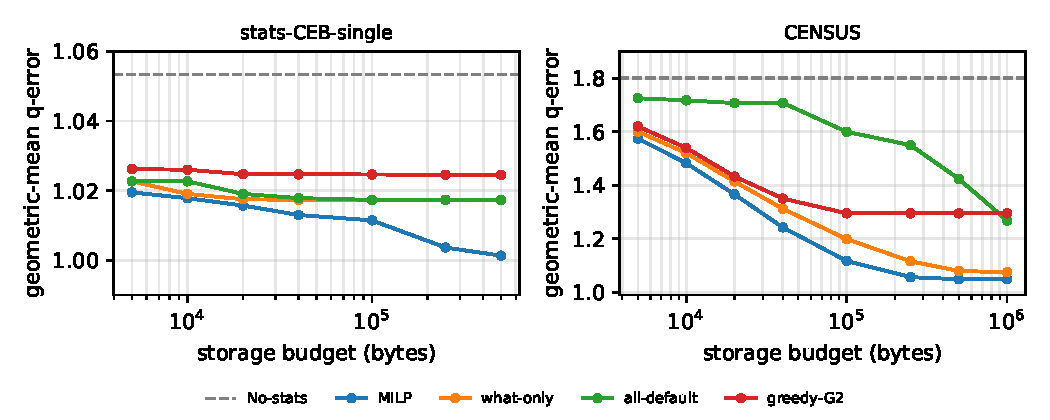
\includegraphics[width=\linewidth]{figures/sec6_rq2}
\caption{Geometric-mean q-error (lower is better) vs.\ storage budget
(log scale) on both primary workloads, for our MILP and the three baselines
(\S\ref{sec:setup}). ``No-stats'' is the constant baseline without
statistics.}
\label{fig:rq2}
\end{figure}

Figure~\ref{fig:rq2} shows the geometric-mean q-error on both workloads across
budgets. On \textsc{stats-CEB-single}, the MILP improves the geometric mean from
$1.05$ (baseline) to $\le1.02$ at 5\,KB and $1.001$ at 500\,KB, and always
dominates the baselines; on the heavy-tailed CENSUS workload it drops the
geometric mean from $1.80$ to $1.05$ by 500\,KB while the worst q-error falls
from $4{,}162$ to $2.85$. The marginal greedy and the naive
\texttt{All-default} practice lag clearly, and their advantage (like that of
the what-only ablation) saturates because neither can reallocate a tight budget
toward capacity (\S\ref{sec:rq3}).

Under every tested storage budget, our joint what-and-how-much MILP solution yields lower q-error compared with the naive \texttt{All-default-candidates} baseline and the marginal greedy baseline.
Larger storage budgets generally enable further estimation-quality improvements, yet marginal returns diminish as budget grows.
The quality advantage of our MILP is most pronounced under tight storage budgets, where resource allocation becomes critical.

\begin{quote}
\noindent\textbf{Answer to RQ2}:
Under identical storage-budget constraints, our joint what-and-how-much MILP optimization outperforms naive practical tuning strategies and knapsack-style greedy baselines on real-world workloads and achieves superior cardinality-estimation quality.
\end{quote}

\subsection{RQ3: Ablation study: benefit of joint what-and-how-much optimization}
\label{sec:rq3}

RQ3 quantifies the performance gains originating from the \textit{how-much} dimension, i.e., differentiated per-statistic sample-size assignment.
We contrast our full MILP model against the what-only ablation baseline, which selects column-sets but assigns a uniform global sample-size for every selected statistic.

Table~\ref{tab:whathowmuch} reports, on the full 632-query workload, the
full model's geometric-mean / maximum q-error against the what-only ablation
(every selected statistic locked to sample size $100$). The capacity-aware
model is never worse and, at 250--500\,KB, drives the maximum from $2.19$ (where
the fixed-capacity baseline saturates) down to $1.45$/$1.17$ by spending the
budget \emph{upgrading} the dominant combinations' capacity instead of adding
more coverage.

\begin{table}[t]
\caption{What-only (fixed capacity, sample size $100$) vs.\ what+how-much
(capacity-aware) MILP on the 632-query workload: geometric-mean and maximum
q-error per budget.}
\label{tab:whathowmuch}
\small
\begin{tabular}{lcc@{\hskip 6pt}cc}
\toprule
 & \multicolumn{2}{c}{what+how-much} & \multicolumn{2}{c}{what-only}\\
\cmidrule(lr){2-3}\cmidrule(lr){4-5}
budget & gmean & max & gmean & max\\
\midrule
5\,\,KB    & \textbf{1.0195} & \textbf{2.22} & 1.0227 & 2.23\\
40\,KB   & \textbf{1.0130} & 2.19 & 1.0173 & 2.19\\
100\,KB  & \textbf{1.0114} & 2.19 & 1.0173 & 2.19\\
250\,KB  & \textbf{1.0036} & \textbf{1.45} & 1.0173 & 2.19\\
500\,KB  & \textbf{1.0013} & \textbf{1.17} & 1.0173 & 2.19\\
\bottomrule
\end{tabular}

{\footnotesize gmean/max = geometric-mean and maximum q-error at that budget.}
\end{table}

Consistent with our insight on two-sided capacity trade-offs, clear performance gaps emerge between the full model and what-only ablation.
The gap is especially prominent under tight budgets: the joint model can re-allocate storage budget to upgrade capacity for high-impact statistics, rather than wasting budget on many low-value statistics with fixed capacity.
Under abundant storage budgets, the gap narrows because sufficient space allows even the what-only variant to deploy high-capacity statistics.

\begin{quote}
\noindent\textbf{Answer to RQ3}:
Non-trivial quality gains originate from the how-much dimension.
Merely selecting promising column-sets with uniform global sample-size cannot capture the full achievable cardinality-estimation improvement, especially under constrained storage budgets.
\end{quote}

\subsection{RQ4: Sensitivity to storage-budget constraint}
\label{sec:rq4}

For RQ4, we vary the input storage-budget parameter and examine three classes of outputs:
\begin{enumerate}
    \item Aggregated estimation quality (geometric-mean / P90 / max q-error).
    \item Composition of the resulting statistic set: total count of selected statistics and distribution of assigned sample-size capacity levels.
    \item MILP solver runtime behaviour across different budget configurations.
\end{enumerate}

% TO-BE-SUPPLEMENTED: insert sensitivity plots: (1) q-error versus storage budget; (2) statistic count and capacity-level mix over budget; (3) MILP solving runtime; record conditions where solver timeout triggers.
% Supplement full-workload end-to-end wall-clock time for Catalog-Mask measurement.

\emph{Quality vs.\ budget.} Figure~\ref{fig:rq2} (right panel) shows the
CENSUS quality curve: a tiny budget already collapses its catastrophic
baseline (geometric mean $25.19\!\to$ arithmetic; maximum $4{,}162\!\to$), and
the curve \emph{saturates} near $\approx$500\,KB (CENSUS geometric mean plateaus
at $\approx1.05$). \emph{Composition.} The selected statistic count grows with
budget --- CENSUS selects 15 statistics at 5\,KB, 206 at 100\,KB, and 455 at
500\,KB, beyond which it stays $\approx$457 while quality is flat, confirming
saturation. The capacity-level mix is opposite in character on the two
workloads: \textsc{stats-CEB-single} shifts to \emph{high} capacity (L1000/
L10000) as the budget grows, whereas data-capped CENSUS spends on
\emph{low} capacity (L10/L25) because its low-cardinality combinations are
already full.

\emph{Solve runtime.} Table~\ref{tab:sec6solve} reports MILP solve time and the
resulting statistic count per budget. \textsc{stats-CEB-single} ($2{,}116$
variables) solves in under a second at every budget. CENSUS is substantially
larger ($159{,}158$ variables; the pruned scale of \S\ref{sec:scale}): the
tightest 5\,KB budget takes $\approx$54\,s, but the solve time drops to
$2$--$4$\,s as the budget loosens, because a tighter feasible region forces more
branch-and-cut to prove optimality. The 300\,s solver timeout is never reached.

\begin{table}[t]
\caption{MILP solve time (seconds) and selected-statistics count vs.\ storage
budget on both primary workloads (same machine as \S\ref{sec:setup}).}
\label{tab:sec6solve}
\small
\begin{tabular}{lcc@{\hskip 6pt}cc}
\toprule
 & \multicolumn{2}{c}{\textsc{stats-CEB-single}} & \multicolumn{2}{c}{CENSUS}\\
\cmidrule(lr){2-3}\cmidrule(lr){4-5}
budget & solve (s) & \#stats & solve (s) & \#stats\\
\midrule
5\,\,KB     & 0.16 & 6   & 54.2 & 15\\
40\,KB    & 0.36 & 10  & 10.4 & 96\\
100\,KB   & 0.80 & 23  & 3.4  & 206\\
250\,KB   & 0.44 & 18  & 4.3  & 380\\
500\,KB   & 0.44 & 33  & 4.5  & 455\\
1000\,KB  & --- & --- & 2.3 & 457\\
\bottomrule
\end{tabular}

{\footnotesize ``---'' = budget not evaluated for \textsc{stats-CEB-single}.}
\end{table}

\emph{Measurement vs.\ optimization.} As \S\ref{sec:scale} and \S\ref{sec:measure-runtime}
detail, the pipeline's dominant cost is the Catalog-Mask candidate-$\times$-
capacity measurement, not the MILP: on CENSUS, phase-1 measurement takes a
comparable workload-wide wall-clock of tens of minutes to hours, while the
optimization is at most a minute. This separation justifies treating
measurement --- not integer programming --- as the bottleneck, and motivates the
Catalog-Mask protocol of \S\ref{sec:measure}.

As storage budget increases, our solver tends to select more column-set candidates and assigns larger sample-size capacity to high-benefit statistics.
Once budget exceeds a saturation threshold, further increasing storage brings negligible additional quality improvement, as most high-value correlation combinations have already been adequately covered.

We also confirm that MILP solving itself is computationally cheap.
The dominant time cost of our overall pipeline lies in Catalog-Mask candidate-$\times$-capacity measurement phase rather than integer-programming optimization.

\begin{quote}
\noindent\textbf{Answer to RQ4}:
Storage-budget strongly influences both estimation quality and the final statistic deployment configuration.
Marginal quality returns diminish once budget crosses a saturation threshold.
Optimization runtime remains manageable; measurement is the major pipeline bottleneck.
\end{quote}

\subsection{Section Summary}
In this section, we report evaluation results obtained under Catalog-Mask's interference-free oracle measurement.
We verify the prevalence and characterize the failure boundary of one-stat sufficiency over real-world and synthetic workloads.
Our joint what-and-how-much MILP optimization outperforms naive practical tuning and greedy algorithmic baselines.
Controlled ablation validates the critical contribution brought by per-statistic sample-size tuning (the how-much dimension).
We further analyse solution sensitivity with respect to storage-budget input and identify measurement as the main computational bottleneck of our pipeline.

Real-system deployment effects including planner interference triggered by overlapping co-installed statistics are deferred to Section~\ref{sec:end2end}.

\section{End-to-End Validation}
\label{sec:e2e}
\label{sec:end2end}

We close the loop of the measurement $\to$ optimization $\to$ deployment
pipeline by building the MILP-selected sets on the real database. Our
measurement model (\S\ref{sec:measure-correct}) makes two predictions:
(a) an isolated measurement should be exactly predictive, and (b) co-installed
overlapping statistics should not affect each other. We test both causally in
three stages --- single-statistic predictability, co-installed predictability,
and restoring predictability --- each stage controlling the previous.

\subsection{Isolated Measurements Are Predictive}
\label{sec:e2e-singleton}

We first confirm that the mask-measured q-error of a single statistic matches
what it delivers when deployed alone. For the statistic
\texttt{posts(AnswerCount,}\allowbreak\texttt{FavoriteCount,}\allowbreak\texttt{ViewCount)} the catalog-mask measurement
predicts q-errors of 1.042 / 1.029 / 1.025 for queries st.144 / st.588 / st.284.
Building \emph{only} that statistic and re-measuring on the real table gives
1.042 / 1.029 / 1.025 --- matching the prediction exactly. This is the
grounding for \S\ref{sec:measure-correct}: per-candidate measurement is sound,
and it validates the economic premise of the whole pipeline (measure each
candidate in isolation, then compose).

\subsection{Overlap Breaks the Independence Assumption}
\label{sec:e2e-coinstalled}

Next we deploy the 2 MB MILP solution for stats\_\allowbreak CEB\_single: five statistics,
all pairwise-overlapping MCVs over \{AnswerCount, FavoriteCount, ViewCount,
PostTypeId\}, predicted mean q-error 1.021. Measured on the real table the mean
is \textbf{1.32} --- a 1.29$\times$ gap. Five of the eight queries match their
prediction (st.562: 1.003, st.308: 1.000, st.182: 1.000, st.398: 1.060, st.314:
1.008), but the three queries served by the \emph{same} statistic
\texttt{(AnswerCount,}\allowbreak\texttt{FavoriteCount,}\allowbreak\texttt{ViewCount)} degrade from their Stage-1
predictions (1.042/\allowbreak1.029/\allowbreak1.025) to 2.13 / 2.07 / 1.90.

Compare Stage 1 and Stage 2 for the very same statistic: alone it delivers
1.042; co-installed with four overlapping siblings it gives 2.13.
The \emph{statistic did not change, and its measurement was exact} (Stage 1);
what changed is that the planner now uses \emph{a different} overlapping
statistic --- a second-order interaction among co-installed statistics, exactly
the independence assumption the per-candidate sparse model relies on, and a
joint effect the per-candidate measurement cannot see by construction.

\emph{Why overlap breaks predictability: creation order.} \label{sec:switch}
To verify this optimizer-internal claim directly, we instrument \texttt{EXPLAIN}
on seven overlap-prone queries: for each we take a pair of overlapping
statistics (A = the good one, B = a bad sibling sharing columns) and read the
planner's estimate under three mask conditions --- B-only, A-only, and both live
(A created \emph{before} B, as in a normal deployment). In every case the
co-installed estimate is \emph{bit-identical} to A-only, never a blend and
never B. Crucially, this is \emph{not} because the optimizer ``picks the better
statistic'': the planner traverses its per-relation statistic list in OID
order, which in our deployments matches creation order, and uses the
\emph{first} matching statistic, so building the same pair with B first flips
the winner purely by swapping creation order. Thus, in our instrumented cases,
the co-installed estimate depends on which statistic the planner happens to
reach first rather than on which is intrinsically better; this explains why
overlap can invalidate isolated measurements even when each isolated
measurement is correct. Disjoint deployments (Stage 3) restore predictability
because with no overlapping pairs the ``first-built'' choice is forced.

\subsection{Disjointness Restores Predictability}
\label{sec:p1}

We fix the gap with the Option-A model: a \emph{global-disjointness} constraint
($y_a+y_b\le 1$ whenever the column sets of $a,b$ overlap) forces the deployed
set to be pairwise column-disjoint, so the planner cannot cross-talk. Table
\ref{tab:p1} measures predicted vs E2E for both models at two budgets.

\begin{table*}[t]
\caption{Three-stage causal summary and Option-A ablation. Ratio $=$
E2E$/_{}$predicted q-error; $1.000$ means the deployment reproduces its
prediction exactly.}
\label{tab:p1}
\small
\begin{tabular}{lccccc}
\toprule
deployment & budget & stats & predicted & E2E & ratio\\
\midrule
singleton (Stage 1)      & --    & 1 & 1.02--1.04 & 1.025--1.042 & $\approx$1.000\\
co-installed overlap (Stage 2) & 2 MB & 5 & 1.021 & 1.320 & 1.294\\
global-disjoint (Stage 3) & 2 MB & 2 & 2.004 & \textbf{2.004} & \textbf{1.000}\\
overlap allowed & 100 KB & 7 & 1.632 & 1.933 & 1.184\\
global-disjoint & 100 KB & 2 & 2.004 & \textbf{2.004} & \textbf{1.000}\\
\bottomrule
\end{tabular}

{\footnotesize predicted = model-predicted q-error; E2E = measured on the real table.}
\end{table*}

Across the deployments we ran, the global-disjoint solution is
\emph{exactly} predictable (ratio 1.000 at both budgets), because the deployed
set is pairwise column-disjoint so the planner cannot cross-talk --- the
independence assumption holds \emph{structurally}, not per-query. The cost of
disjointness is a well-defined nominal-quality loss (predicted 2.00 vs.
1.02): it forces the solver to forgo overlapping-but-high-value dominant
candidates.

\emph{Generality across many deployments.} To show this is not an artefact of a
hand-picked deployment, on the real \texttt{posts} table we deploy 5 singletons
plus the whole-workload budgeted MILP at four budgets (10/40/100/250\,KB), each
solved both \emph{with} global disjointness and \emph{without}, and measure E2E
for every query a deployment touches; \label{sec:e2esys}
Fig.~\ref{fig:e2epredict} summarizes 234 disjoint (159 global-disjoint MILP $+$
75 singletons) and 230 overlapping query-deployment points.

\begin{figure}[t]
\centering
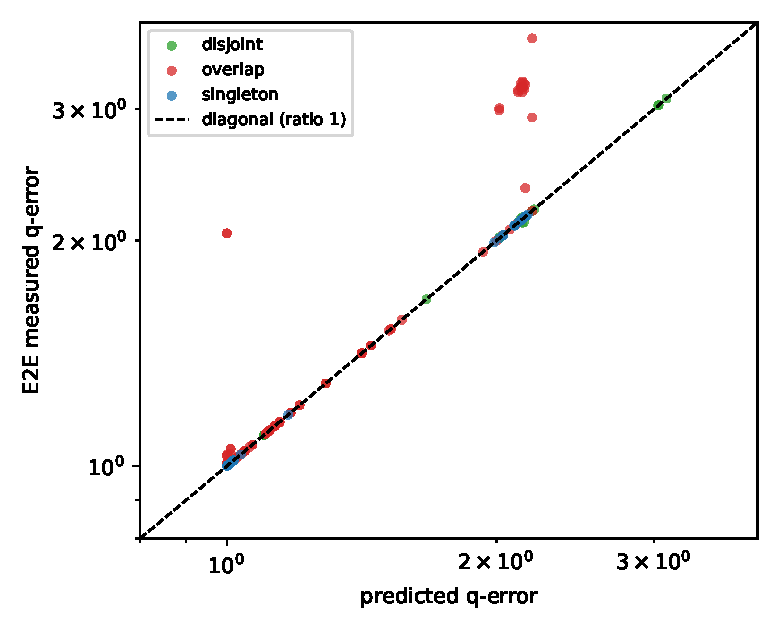
\includegraphics[width=\linewidth]{figures/e2e_predict}
\caption{Predicted vs.\ E2E measured q-error across 464 systematic
query-deployment points (log-log). Disjoint points are singletons and
global-disjoint MILP deployments; overlapping points are unconstrained
deployments.}
\label{fig:e2epredict}
\end{figure}

The sweep confirms the Stage-2/3 finding is \emph{not} an artefact of a
hand-picked deployment: disjoint deployments reproduce their predictions to
within $1.001$ at every budget (only 8 of 159 global-disjoint points exceed a
ratio of $1.0001$; mean $1.0000$, worst $1.036$), while overlapping
deployments, on average, exceed theirs --- the mean ratio is tightest at the
largest budget ($1.018$ at 250\,KB) and largest under small budgets where
overlap is densest ($1.07$--$1.08$ at 10/40\,KB). The residual is a \emph{tail}
rather than a uniform shift: the median overlapping ratio is $1.000$, only
$20/230$ overlapping points exceed $1.05$ --- but those can be severe (worst
$2.05$). This is exactly what a per-candidate measurement model predicts:
individual statistics are faithful, and the residual error is a joint effect of
co-installed overlapping statistics that disjointness removes --- and removes
\emph{generally}, not just in the original two deployments.

\subsection{The Causal Takeaway}
\label{sec:e2e-takeaway}

Together, the three stages show that isolated measurements are predictive,
while co-installed overlapping statistics introduce the residual interaction;
global disjointness removes it at a quantified quality cost. Option~B remains
available when that quality cost is unacceptable, but requires post-selection
validation (\S\ref{sec:disc-fix}).

\section{Discussion and Open Questions}
\label{sec:disc}

\subsection{A Mechanistic Interpretation}
\label{sec:disc-sparsity}

A single-table selection query's error is typically dominated by \emph{one}
correlated column cluster: its restriction is a conjunction of predicates whose
selectivity error is largest where independence fails hardest, so a single MCV
over that dominant cluster removes the dominant error source while
weakly-correlated residuals contribute little. This mechanistically explains
one-stat sufficiency and its boundary: workloads genuinely driven by
\emph{several} independent clusters violate it and warrant the multi-select
model (\S\ref{sec:formulation}), as our stress test confirms
(Table \ref{tab:sweep}); characterising how often that regime occurs is an open
question below.

\subsection{What Is Being Optimized}
\label{sec:disc-objective}

We optimize a \emph{storage} budget (persistent bytes and estimation quality,
\S\ref{sec:rq3}); ANALYZE maintenance cost is treated separately because
PostgreSQL couples sampling effort to the \emph{maximum} target on a relation
(\S\ref{sec:mechanisms}); a maintenance-aware variant is an open question
below. The budget-quality curves (\S\ref{sec:rq3},
Fig.~\ref{fig:rq2}) show the budget is, in practice, spent on the
``how much'' axis. A DBA often values the \emph{maintenance} burden over
persistent size, and here one-stat sufficiency helps directly: because each
query needs at most one dominant statistic (\S\ref{sec:rq1}), the selected set
is \emph{small}, so both the number of objects to create and the ANALYZE volume
to refresh them stay low --- maintenance cost is reduced by construction.

\emph{The resulting storage/ANALYZE mismatch.} Because storage is additive
while ANALYZE cost is a property of each relation's \emph{maximum}
\texttt{statistics\_target}, the two can diverge sharply. A \emph{data-capped}
statistic (\S\ref{sec:rq4}) at L10000 stores the same bytes and yields the same
q-error as its L1000 twin, yet it forces PostgreSQL to sample ANALYZE at target
10000 (a $10\times$ larger sample). Quantitatively, at a 100\,KB budget on
stats\_CEB\_single, the storage-only MILP solution and one capped at L1000 have
identical storage (99{,}996 B) and identical mean q-error (1.0156), but
reconstructing them by ANALYZE differs by $\approx$2.7$\times$ (31.4\,s vs.\
11.6\,s). The storage-only
objective is thus a genuine but imperfect proxy for maintenance cost; a
maintenance-aware objective (open question~1) is the natural extension.

\emph{Why arithmetic mean q-error.} We use arithmetic mean q-error because it
emphasizes the heavy error tail while preserving the linear MILP objective. A
log-objective produces nearly identical mean q-error across budgets, indicating
that the main conclusions are not sensitive to this choice.

\subsection{Deployment Fidelity of the Oracle}
\label{sec:disc-deployment}

This issue is distinct from the planner-interference of \S\ref{sec:e2e}: the
former concerns \emph{how a statistic is sampled at a given target}
(large-sample oracle vs.\ a real target-specific deployment), the latter
\emph{which statistic the planner uses when several are co-installed}.

Protocol-M evaluates every capacity level on the same large sample (a
\emph{large-sample oracle}), which a real ``\texttt{SET STATISTICS} $L$''
deployment need not reproduce. Target-specific ANALYZE shows high fidelity on
the evaluated \texttt{stats\_CEB\_single} candidates and the core \texttt{posts}
case: the oracle-selected level incurs at most 1\% q-error loss relative to the
true best level, and the headline $4.58\to2.82\to1.04$ curve is reproduced
within 1\%. In the low-$\lambda$ cases we evaluated, however, the oracle is
optimistic: when the candidate covers a rare-selectivity driver but the
combination is too rare to appear in a real low-capacity sample, the large
sample captures it while a real small sample falls back to base-frequency with
a far worse q-error; the real/oracle ratio reached $\sim$$10^{2}{-}10^{4}$ and
approached 1 once $\lambda$ was several units or larger
($\lambda(L){=}(r/N)\cdot\textrm{sample}(L)$ the expected sample count). We
treat low expected counts as an \emph{empirical warning regime}, not a hard
threshold.

\subsection{The Interference Fix}
\label{sec:disc-fix}

The validated fix (Option A, global disjointness) is the trustworthy main model:
it restores empirically near-exact predictability at a quantified quality cost
(\S\ref{sec:p1}). As a practical fallback (Option B), one can solve without the
constraint and then repair the deployed set. Table~\ref{tab:optionB} measures
both modes end-to-end on the real \texttt{posts} table across three budgets,
reporting the achieved arithmetic-mean q-error over the whole workload and the
number of queries whose E2E/predicted ratio exceeds $1.05$ (``tail'').

\begin{table}[t]
\caption{Option-A vs.\ Option-B end-to-end on the real \texttt{posts} workload
at three budgets. \emph{mean} = achieved arithmetic-mean q-error over the
workload; \emph{tail} = queries with E2E/predicted ratio $>1.05$ (out of
served).}
\label{tab:optionB}
\small
\setlength{\tabcolsep}{2.6pt}
\begin{tabular}{lcccccc}
\toprule
deployment & \multicolumn{2}{c}{40\,KB} & \multicolumn{2}{c}{100\,KB} & \multicolumn{2}{c}{250\,KB}\\
\cmidrule(lr){2-3}\cmidrule(lr){4-5}\cmidrule(lr){6-7}
 & mean & tail & mean & tail & mean & tail\\
\midrule
\textsf{overlap} (unconstrained) & 1.031 & 8/48 & 1.024 & 5/75 & 1.006 & 1/64\\
Option-A disjoint & 1.042 & \textbf{0}/32 & 1.042 & \textbf{0}/41 & 1.042 & \textbf{0}/50\\
Option-B repaired & 1.030 & 7/50 & 1.026 & 4/46 & 1.020 & 6/50\\
\quad (iterated) & 1.031 & 7/50 & 1.025 & 4/46 & 1.019 & 3/63\\
\bottomrule
\end{tabular}
\end{table}

The two modes make an honest, complementary trade. Option~B \emph{preserves the
nominal quality} of the unconstrained solution --- its achieved mean q-error
($1.019$--$1.031$) is close to the overlap baseline and far better than
Option~A's $\approx\!1.04$ --- but it does \emph{not} eliminate the
predictability tail: dropping the flagged statistics and re-solving fixes the
originally-scary queries yet introduces new interfering pairs as the solver
re-opens the budget, so the residual tail never reaches zero
(Table~\ref{tab:optionB}). Option~A is the only mode with \emph{zero} tail at
every budget, at the price of the quality gap. We recommend A as the default
because it makes the deployment semantics match the measurement model
(\S\ref{sec:measure-correct}) --- the deployment is then structurally
independent, not just measured independently --- and reserve Option~B for
deployments where quality outranks the reproducibility guarantee, expecting to
repeat the solve $\to$ EXPLAIN-check $\to$ drop $\to$ re-solve loop since the
interference is emergent rather than a fixed set of bad statistics.

\subsection{Open Questions}

(1) \emph{Maintenance-aware selection}: jointly modeling ANALYZE cost (a function
of the \emph{max} target) would replace the storage-only budget with an
end-to-end maintenance budget. (2) \emph{When does one-stat sufficiency fail?:}
identifying workloads with genuinely multiple independent correlated clusters
(the regime needing the multi-select model, \S\ref{sec:formulation}) is the
most important open question. (3) \emph{Higher-order candidates}: our
2-/3-column candidate family understates achievable quality on harder CENSUS
queries, where 4-/5-column MCVs help --- extending candidate generation to
higher arity is future work.

\section{Conclusion}
\label{sec:concl}

Extended-statistics selection should be treated as a joint \emph{which} and
\emph{how much} decision. On the two single-table workloads we evaluate
(stats\_CEB\_single and the wide CENSUS benchmark) we observe one-stat
sufficiency among the evaluated 2-/3-column MCV candidates --- at most one
dominant statistic per query --- which, together with capacity levels, makes the
budget-constrained problem an exactly-linear MILP solvable in seconds at
full-workload scale, via
a catalog-mask protocol that makes per-candidate, per-capacity measurement
feasible on wide tables. End-to-end validation confirms the correctness of
\emph{isolated} per-candidate measurement and identifies two distinct
deployment risks: sampling mismatch in rare low-frequency regimes
(\S\ref{sec:disc-deployment}) and planner cross-talk among co-installed
overlapping statistics; we explain the latter as a creation-order effect
(\S\ref{sec:switch}) and restore empirically near-exact predictability either
with a conservative global-disjointness mode or with post-selection
planner-validation. Join-heavy workloads are the negative control.

\emph{Scope.} We state precisely what we do and do not claim. Our contribution
is not an MILP \emph{per se}, nor a claim that extended-statistics selection is
inherently sparse. It is the combination of three scoped findings: (i) a
\emph{capacity-aware} reformulation --- the ``what $\times$ how much'' budget
allocation across \texttt{statistics\_target} --- which is new and independent
of sufficiency; (ii) a \emph{measurable one-stat sufficiency}, characterized
empirically on the two evaluated single-table workloads (with an explicit,
synthetic demonstration of where it fails); and (iii) a \emph{scalable
measurement} protocol that turns the candidate $\times$ capacity space into data
the optimizer can consume. Taken together --- not any single one --- these make
capacity-aware extended-statistics selection \emph{optimizable and
deployable} on the workloads we evaluate; the general (Boolean-multi-select,
arbitrary-statistic-kind, join-dominated) version of the problem is explicitly
out of scope.

\begin{acks}
\emph{Acknowledgements.} (to be completed)
\end{acks}

\bibliographystyle{ACM-Reference-Format}
\bibliography{references}

\end{document}
\endinput
